\section{Struktur Organisasi}

Bangkit didesain untuk mempersiapkan peserta dengan kecakapan (skills) yang relevan dan dibutuhkan berdasarkan sertifikasi teknikal. Tahun ini Bangkit kembali menyelenggarakan 3 (tiga) alur belajar multidisiplin -\textit{ Machine Learning, Mobile Development (Android)}, dan \textit{Cloud Computing}. Dengan mengikuti Bangkit, peserta akan memiliki pengalaman dan terekspos dengan serba-serbi karir di industri dan pekerjaan di ekosistem teknologi Indonesia.

Bangkit merupakan program pembelajaran yang dipimpin oleh \textbf{Google} dengan dukungan \textbf{GoTo, Traveloka,} dan \textbf{DeepTech Foundation}. Dengan dukungan Kampus Merdeka, Bangkit akan menawarkan 3.000 tempat untuk mahasiswa Indonesia untuk memastikan mereka relevan dengan kecakapan yang dibutuhkan oleh industri pada semester genap, tahun 2021/2022.

Adapun struktur organisasi merupakan sebuah garis penugasan formal yang menunjukkan alur tugas dan tanggung jawab setiap anggota perusahaan, perusahaan serta hubungan antar pihak dalam organisasi yang bekerja sama untuk mencapai suatu tujuan organisasi. Struktur organisasi dari Bangkit Academy.

\begin{figure}
    \centering
    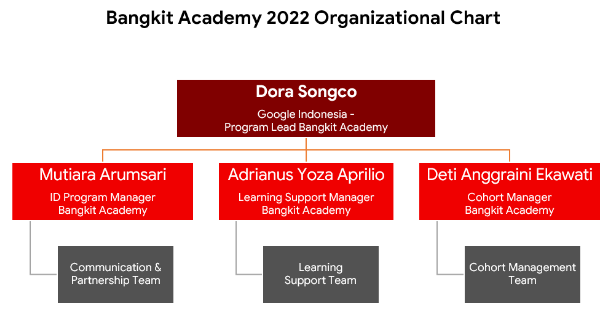
\includegraphics[width=\textwidth]{chapters/images/bangkit-2022-org-diagram.png}
    \caption{\textit{Bangkit Academy 2022 Organizational Chart}}
    \label{fig:gambar3.1}
\end{figure}

\section{Lingkup Pekerjaan} \label{lingkup-pekerjaan}

Bagian \textit{learning path cloud computing}, yaitu \textit{path} yang saya pribadi ambil dalam program ini membahas mengenai utilisasi dari \textit{cloud}, secara esensinya adalah \textit{server} yang dapat diakses oleh internet yang dibagi menjadi dua bagian besar \textit{private} dan \textit{publik}, secara spesifiknya dalam program ini, siswa \textit{cloud computing} diharapkan dapat menggunakan \textit{cloud platform} milik \textbf{Google} yaitu \textbf{GCP} atau \textbf{Google Cloud Platform}, serta memahami hal-hal teknis yang perlu diketahui untuk menggunakan \textit{cloud platform} secara efektif.

Melihat proyek yang telah dilakukan, hal ini berkaitan mengenai \textit{infrastructure} dan \textit{architecture planning}, yang dilakukan pada saat tahap \textit{pre-working} dalam proyek. Pengintegrasian \textit{services} pada tahap pengerjaan, serta pada akhirnya mendapatkan aplikasi yang bekerja secara sepenuhnya pada tahap \textit{post-working}.

\section{Deskripsi Pekerjaan}

Masuk ke topik lingkup yang sudah dibahas secara sekilas pada \ref{lingkup} kegiatan dalam program baik dalam program yang saya jalani; \textit{cloud computing}, serta \textit{learning path} lainnya (dengan perbedaan material dan \textit{provider} pada \textit{self-paced course}), terdiri dari empat kategori besar, dengan tiga dari empat kegiatan yang dimaksud bersifat wajib dan satu kategori kegiatan tidak bersifat wajib.
\begin{itemize}
    \item \textit{Self-paced Courses}: Yang terdiri dari kursus yang diambil dari tiga \textit{provider} (\textbf{Dicoding}, \textbf{Coursera} dan \textbf{Qwiklabs}), setiap kursus memiliki materi yang perlu dipelajari oleh siswa dengan tenggat waktu yang sudah ditentukan.
    \item \textit{Technical dan Soft-Skill Intructor Led Training / ILT}: Adalah pelatihan yang bekerja sebagai pengantar untuk \textit{self-paced course} (untuk \textit{ILT Tech}) dan sebagai pelatihan untuk keahlian \textit{soft-skill} (di dalamnya termasuk Bahasa Inggris), dipimpin oleh seorang instruktur yang memiliki pengalaman dalam bidangnya dan memiliki tugas pada setiap akhir \textit{ILT}.
    \item \textit{Capstone Project}: Sebuah proyek akhir yang dimana setiap peserta menggunakan keterampilan yang didapat dari program untuk membuat sebuah aplikasi dengan tema tertentu.
    \item \textit{Challenges, Guest Speakers} dan konsultasi: Sebuah tantangan yang berkaitan dengan keterampilan spesifik \textit{soft-skill} dan sesi \textit{guest speaker} dengan materi yang bervariasi. Kedua kegiatan yang disebutkan adalah \textbf{opsional}.
\end{itemize}
Setiap \textit{learning path} memiliki seluruh kegiatan yang disebutkan di atas (minus \textit{provider} tertentu dalam \textit{self-paced course}, dan diharapkan dapat menyelesaikan kegiatan-kegiatan di atas berdasarkan waktu yang telah ditentukan dalam jadwal diikuti dengan nilai yang cukup. Khusus untuk \textit{ILT}, yang wajib diikuti oleh seluruh \textit{cohort} atau siswa dalam program ini hanya dapat diikuti dengan waktu tertentu yang sudah diberikan. Siswa hanya sebatas memiliki kewajiban \textbf{menghadiri} dan \textbf{menyelesaikan tugas} yang diberikan.

\section{Jadwal Kerja}

Jadwal pada program \textbf{Bangkit 2022} memiliki acuan yang telah ditetapkan dari pihak managemen yang dapat di akses oleh seluruh anggota organisasi (siswa, dan pengurus). Jadwal pembelajaran aktif mulai dari pukul \textbf{09.00-21.00}, yang memuat rentang waktu di mana \textit{team meeting, ILT}, dan konsultasi dapat dilakukan, dan jadwal pasif (jadwal di mana siswa dapat melakukan aktivitas kursus) sepenuhnya diatur oleh siswa.

Sedangkan jadwal keseluruhan yang memuat \textit{rundown} topik yang akan dibahas pada kursus, dan \textit{ILT} dapat dibagi menjadi 5 tahap, dengan 3 tahap awal ditentukan dengan \textit{milestone} yang memiliki rentang satu sampai paling banyak empat minggu, dan dua sisanya merupakan tahap \textit{capstone} dan \textit{post-capstone}, dengan ringkasan sebagai berikut:

\begin{enumerate}
    \item Milestone 1: \textit{Web development} dan \textit{JavaScript}
    \item[] 7 Februari 2022 - 7 Maret 2022, membahas mengenai pengembangan web dan bahasa pemrograman \textit{JavaScript}.
    \begin{itemize}
        \item 4 ILT (2 \textit{tech}, 1 soft-skill, 1 english).
        \item Dua buah kursus yang berkaitan dengan topik.
        \item Satu tugas soft-skill.
    \end{itemize}
    \item Milestone 2: \textit{Backend development} dan \textbf{GCP}
    \item[] 14 Maret 2022 - 28 Maret 2022. membahas mengenai pengembangan web lebih tepatnya \textit{Backend} dan pengenalan pada \textbf{GCP}.
    \begin{itemize}
        \item 3 ILT ( 2 soft-skill, dan satu \textit{tech}).
        \item 3 buah kursus yang berkaitan dengan topik.
        \item Satu tugas soft-skill.
    \end{itemize}
    \item Milestone 3: \textit{GCP}
    \item[] 4 April 2022 - 25 April 2022, membahas lebih lanjut mengenai \textbf{GCP}.
    \begin{itemize}
        \item 5 ILT (2 \textit{tech}, 2 soft-skill, satu english.
        \item 3 buah kursus yang berkaitan dengan topik.
        \item Dua buah tugas soft-skill.
    \end{itemize}
    \item \textit{Capstone Project}
    \item[] 9 May 2022 - 13 Juni 2022, mengerjakan proyek akhir.
    \item \textit{Post-capstone}
    \item[] Persiapan sertifikasi \textit{Google associate cloud engineer}, dan materi soft-skill tambahan.
    \begin{itemize}
        \item 3 ILT (satu\textit{tech}, dua soft-skill).
        \item Satu kursus.
        \item Dua tugas softkill
    \end{itemize}
\end{enumerate}